\documentclass{article}
\usepackage{graphicx}
\usepackage[margin=1in]{geometry}
\usepackage[outdir=./]{epstopdf}  					% Avoids errors when input figures
\usepackage[labelsep=period,labelfont=bf]{caption}
%\usepackage{subcaption}

\begin{document}

\begin{figure}[tbph]
	\begin{center}
		\caption{Persistence of the Yield Curve Response to the Target and Path Factors over Subsequent Days}
		\label{fig:persistsym}
		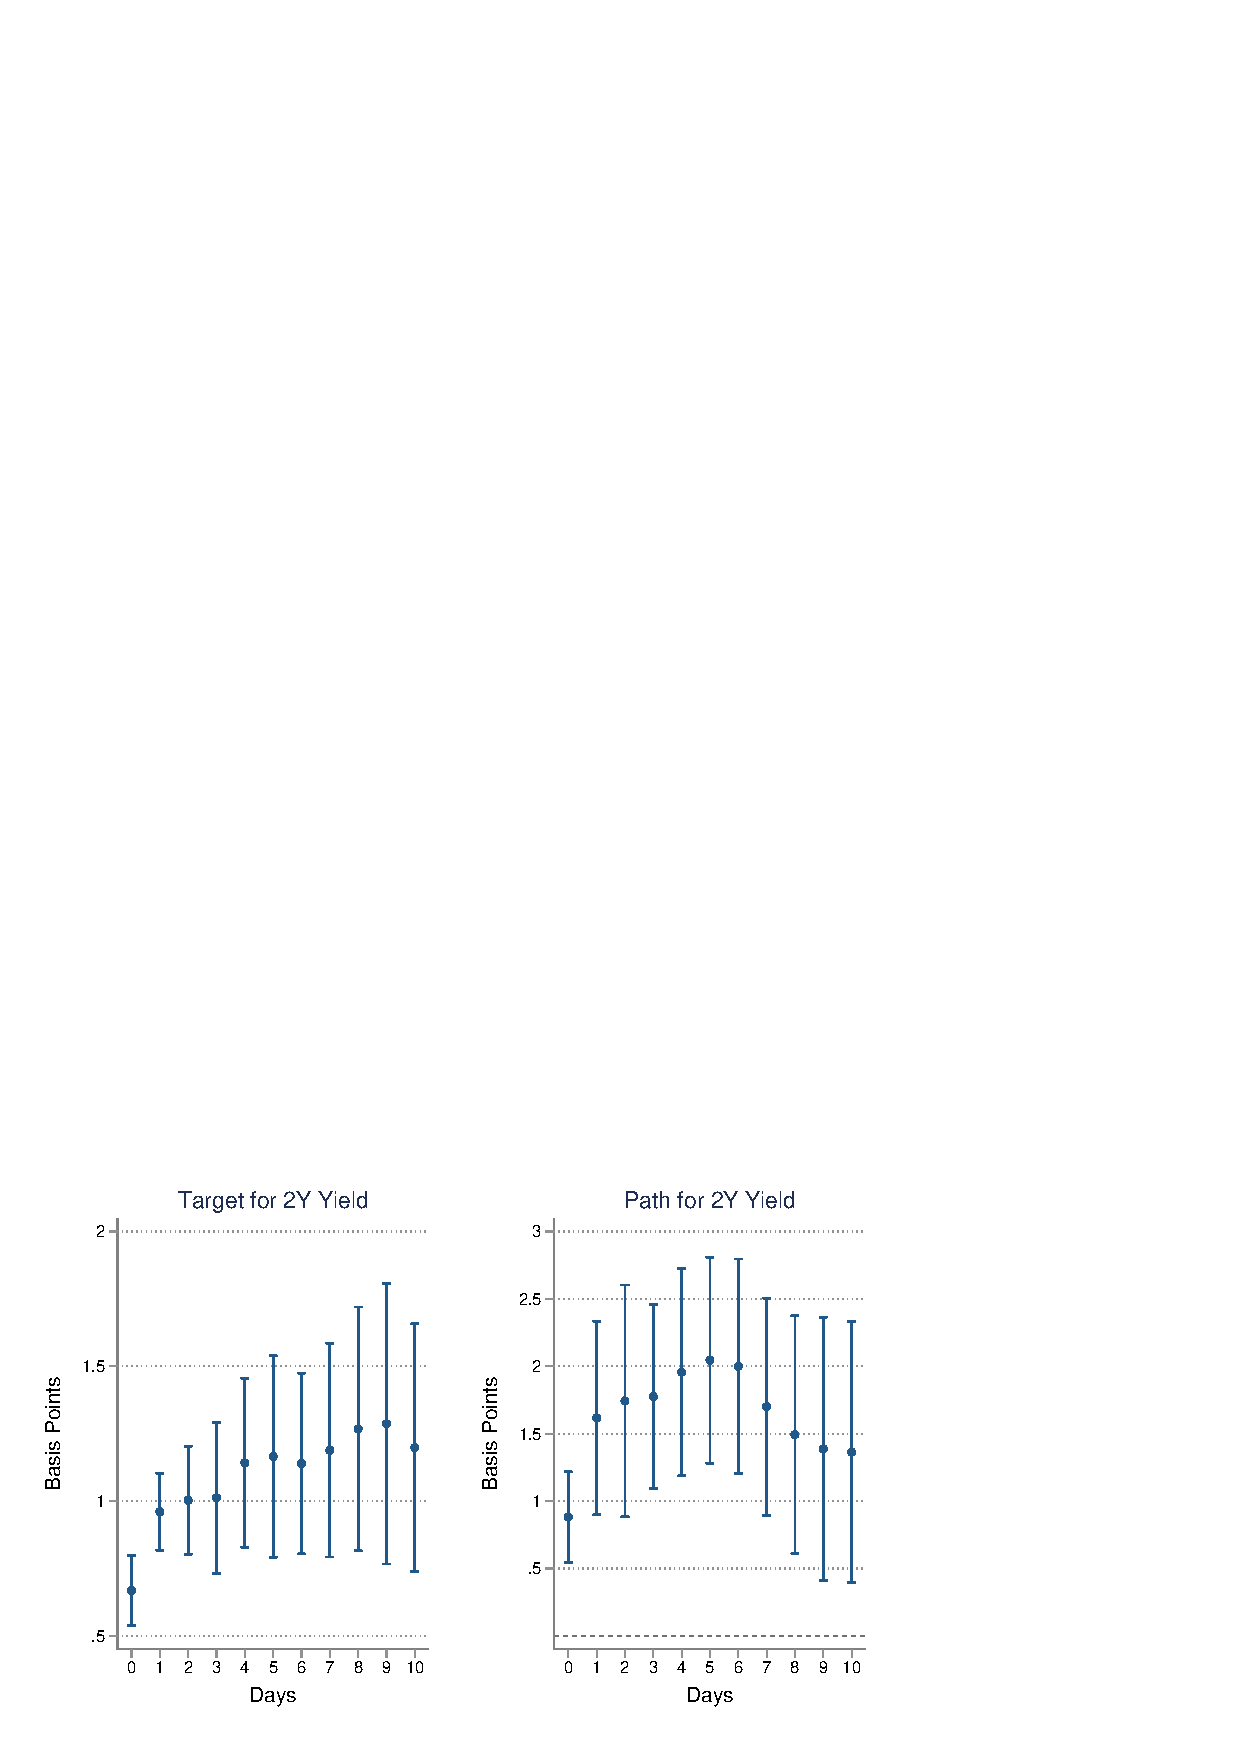
\includegraphics[trim={0.6cm 0cm 0.5cm 0cm},clip,height=.2\textheight,width=1\textwidth]{persistsymgmxn02yr} \\
		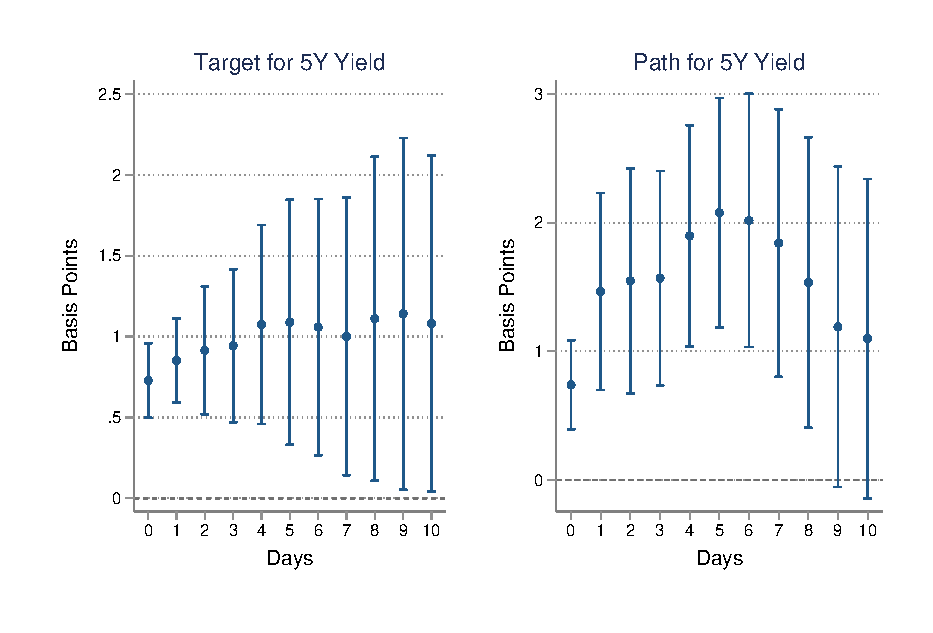
\includegraphics[trim={0.6cm 0cm 0.5cm 0cm},clip,height=.2\textheight,width=1\textwidth]{persistsymgmxn05yr} \\
		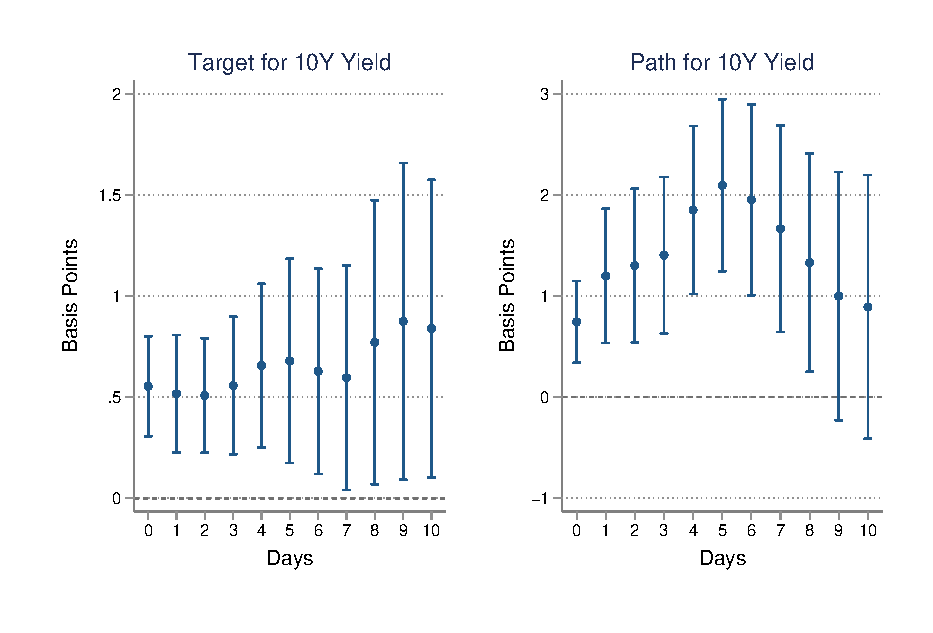
\includegraphics[trim={0.6cm 0cm 0.5cm 0cm},clip,height=.2\textheight,width=1\textwidth]{persistsymgmxn10yr} \\
		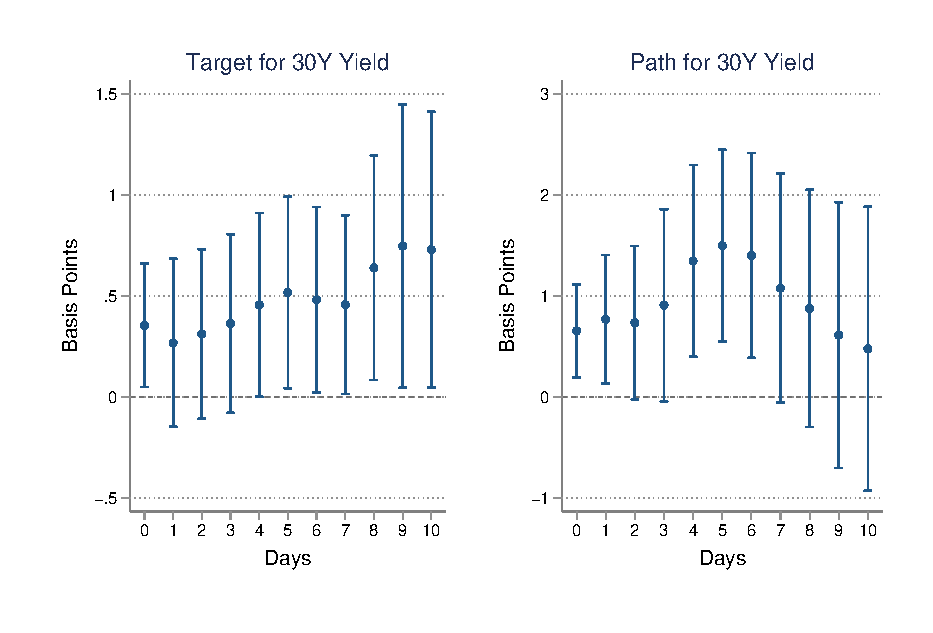
\includegraphics[trim={0.6cm 0cm 0.5cm 0cm},clip,height=.2\textheight,width=1\textwidth]{persistsymgmxn30yr} \\
	\end{center}
	
	\vspace{-0.4cm} \caption*{\footnotesize{\textit{Notes}: This figure plots the coefficient estimates and 95\% confidence intervals for the target (left column) and path (right column) factors obtained from equation (\ref{eq:nTwoFac}) for yield changes from close of day \(t - 1\) to day \(t + k\), where \(t\) is a day with a monetary policy announcement and \(k = 0, 1, \ldots, 10\). The factors are obtained from intraday data, as explain in the main text. The sample is all regular monetary policy announcements from January 2011 to December 2019.}}
\end{figure}

% trim = {<left> <lower> <right> <upper>}

%\begin{figure}[tbph]
%	\caption{Banking Variables for the Banking System.}
%	\label{fig:roa_n_ratios}
%	\begin{subfigure}[t]{\textwidth}
%		\begin{center}
%			\includegraphics[trim={0cm 0cm 0cm 0cm},clip,height=.4\textheight,width=1\textwidth,keepaspectratio]{../../filename} \\
%			\caption{\roa{} Components.} \label{subfig:roadcmp}
%%			\vspace{.5cm}
%		\end{center}
%	\end{subfigure}
%	
%	\begin{subfigure}[t]{\textwidth}
%		\begin{center}
%			\includegraphics[trim={0cm 0cm 0cm 0cm},clip,height=.4\textheight,width=1\textwidth,keepaspectratio]{../../filename} \\
%			\caption{Banking Ratios.} \label{subfig:bankratios}
%%			\vspace{.4cm}
%		\end{center}
%	\end{subfigure}
%	
%	\vspace{-0.4cm} \caption*{\footnotesize{\textit{Notes}: Notes.}}
%\end{figure}

\end{document}
